\documentclass[12pt,letterpaper,oneside]{book}
\usepackage{amsmath, amsthm, amssymb, amsfonts, latexsym, cancel}
\usepackage{geometry}
\usepackage[mathscr]{euscript}
\usepackage{anyfontsize}
\usepackage[spanish]{babel}
\usepackage{shapepar}
\usepackage[utf8]{inputenc}
\usepackage{fancybox}
\usepackage{afterpage}
\usepackage{mathrsfs}
\usepackage{fancyvrb}
\usepackage{fancyhdr}
\usepackage{graphicx}
\usepackage{subfigure}
\usepackage{color}
\usepackage{enumerate}
\usepackage{tikz}
\usepackage{float}
\usepackage{minted}
\usepackage{caption}
\usepackage{subfig}
%\usepackage{subcaption}
%\usemintedstyle{perldoc}
\textheight=21.94cm
\textwidth=15.69cm
\hoffset=-3mm
\pagestyle{headings}
\setcounter{MaxMatrixCols}{30}
\definecolor{verde}{rgb}{0,0,1}
\usepackage[pdftex,colorlinks]{hyperref}
\hypersetup{citecolor=blue,linkcolor=verde}
\usepackage{tensor}
\usepackage[T1]{fontenc}

\usepackage{bm}

\newsavebox\MBox
\newcommand\Cline[2][red]{{\sbox\MBox{$#2$}%
  \rlap{\usebox\MBox}\color{#1}\rule[-1.2\dp\MBox]{\wd\MBox}{0.5pt}}}

\newcommand{\der}[2]{\frac{d #1}{d #2}}
\newcommand{\dder}[2]{\frac{d^2 #1}{d #2 ^2}}
\newcommand{\derp}[2]{\frac{\partial #1}{\partial #2}}
\newcommand{\sch}{Schwarzschild}
\newcommand{\m}{métrica}
\newcommand{\ein}{Einstein}
\newcommand{\la}{\mathcal{L}}
\usepackage{float}

\newcommand\Ccancel[2][black]{\renewcommand\CancelColor{\color{#1}}\cancel{#2}}

%%%%%%%%%%%%%%%%%%%%%%%%%%%%%%%%%%%%%%%%%%%%%%%%%%%%%%%%%%%%%%%%%%%%%%%%%%%%%%%%%%%%%%%%

\usepackage{fancyhdr}
\pagestyle{fancy}
\fancyhf{}
\fancyhead[LO]{\leftmark}
\fancyhead[RO,LE]{\thepage}


%%%%%%%%%%%%%%%%%%%%%%%%%%%%%%%%%%%%%%%%%%%%%%%%%%%%%%%%%%%%%%%%%%%%%%%%%%%%%%%%%%%%%%%%%

\theoremstyle{plain}
	\newtheorem{prop}{Proposición}[section]
	\newtheorem{teor}[prop]{Teorema}
	\newtheorem{corol}[prop]{Corolario}
	\newtheorem{lema}[prop]{Lema}
\theoremstyle{definition}
	\newtheorem{defin}[prop]{Definición}
	\newtheorem{ejem}[prop]{Ejemplo}
\theoremstyle{remark}
	\newtheorem{obs}[prop]{Observación}
	
\renewcommand{\qedsymbol}{$\blacksquare$}
\newcommand{\C}[1]{\left\lbrace #1\right\rbrace}
\newcommand{\ET}{{\small\textsc{T}}}


\newcommand{\algoritmo}[2]{\hrule
\vspace{0.5mm}
\hrule
\hrule
\vspace{0.5mm}
\hrule
\smallskip
{\sc #1 }
\smallskip
\hrule
\smallskip
#2
\smallskip
\hrule
\vspace{0.5mm}
\hrule
\hrule
\vspace{0.5mm}
\hrule}

%%%%%%%%%%%%%%%%%%%%%%%%%%%%%%%%%%%%%%%%%%%%%%%%%%%%%%%%%%%%%%%%%%%%%%%%%%%%%%%%%%%%%%%%%

\begin{document}

\frontmatter

\thispagestyle{empty}
\begin{center}
\textbf{{\LARGE Estudio de la turbulencia fotosférica}}\\[7cm]




\textbf{{\Large Johan Sammir Méndez Holguín}}\\[8cm]

Universidad Nacional de Colombia\\[2mm]
Facultad de Ciencias \\[2mm]
Observatorio Astronómico Nacional\\[2mm]
Bogotá D.C., Colombia\\[2mm]
I Semestre - 2019
\end{center}

\newpage\null\thispagestyle{empty}\newpage


%%%%%%%%%%%%%%%%%%%%%%%%%%%%%%%%%%%%%%%%%%%%%%%%%%%%%%%%%%%%%%%%%%%%%%%%%%%%%%%%%%%%%%%%%%%%%%
\newpage

\thispagestyle{empty}
\label{Portada}
\begin{center}
\textbf{{\LARGE Estudio de la turbulencia fotosférica}}\\[2cm]

Trabajo Final de Pregrado presentado por\\[0.7cm]

\textbf{{\LARGE Johan Sammir Méndez Holguín}}\\[1cm]

al\\[4mm]

{\Large Departamento de Física}\\[1.5cm]

como requisito parcial\\
para obtener el grado de\\[1 cm]

\textbf{{\Large Física}}\\[1.5cm]

dirigido por\\
Phd. Santiago Vargas Domínguez\\
Phd. Miller Mendoza Jímenez\\[1cm]





\includegraphics[scale=.10]{escudo}\\
{\Large Universidad Nacional de Colombia}\\[2mm]
{\Large Facultad de Ciencias}\\[2mm]
Bogot\'a D.C., Colombia\\[2mm]
Junio de 2018

\end{center}

\newpage\null\thispagestyle{empty}\newpage

\newpage
\pagenumbering{roman}
\thispagestyle{empty}
\vspace*{9cm}
\begin{flushright}
\textit{Dedicatoria\\ }
\end{flushright}

\newpage\null\thispagestyle{empty}\newpage

\newpage
\thispagestyle{empty}
\vspace*{3.5cm}

{\Large\textbf{Resumen}}\\

kalakalala

 
 

\textit{Palabras clave: }\\

\bigskip

{\Large\textbf{Abstract}}\\

.\\

\textit{Key words: ...}


\tableofcontents\thispagestyle{empty}
\pagestyle{plain}

\setcounter{page}{1}
\chapter{Introducción}

\medskip





Acá va la introducción al tema, esta parte debe contener de manera clara ciertos temas 

\begin{enumerate}
    \item Dar una relevancia histórica de el tema que se quiere estudiar
    \item describir cada capítulo brevemente 
    \item tratar de esbozar en pocas palabras el estado del arte del tema
\end{enumerate}




  







\medskip

%Quiero hablar de los utiles que son las métricas lo mucho que sirven y como despues de que einstein encontro las ecuaciones de campo se inicio una ardua busqueda para encontrar soluciones y posteriormente para darle sentido fisico\\

%quiero decir que las singularidades tienen me encantan por las complicaciones fisicas que presentan el su existencia y que la existe un teorema que dicen que no se pueden salvar \\

%despues tengo que hecharme un carretaso con geodesicas, \\

%Hay algo que yo creo y es que los discos de acresion de una detterminada métrica podrian darnos a nivel astrofisico la prueba de que si existen estas formas de curvaturas en el espacio tiempo y un primer acercamiento es apartir de las geodesicas.\\


%que por eso mi trabajo recorre desde un formalismo teorico desde el posible significado fisico de mi metrica hasta sus repercusiones en las particulas de prueba .\\



.\\




\mainmatter
\pagestyle{fancy}
\fancyhf{}
\fancyhead[LO]{\leftmark}
\fancyhead[RO,LE]{\thepage}


\setcounter{page}{1}
\chapter{Electrodinámica}

\noindent En la presente sección se revisa la teoría de la  electrodinámica clásica. El estudio de la variación temporal de los campos magnéticos y eléctricos muestra una fuerte relación entre ellos, en donde cambios en los campos eléctricos genera campos magnéticos y viceversa.%\cite{Chaichian}\\

\section{Ley de Gauss}

\noindent Esta es la primera de las ecuaciones básicas para la descripción del campo eléctrico, en donde se hace la deducción de la forma matemática para el campo eléctrico generado a partir de una distribución de cargas en reposo. El campo eléctrico dado por una distribución de cargas está dado por la siguiente expresión \cite{Jackson}

\begin{eqnarray}
    \vec{E}(\vec{r}) =\frac{1}{4\pi\epsilon_{0}} \int_{\bf{V}}\rho(\vec{\bf{r}}
)\frac{\vec{r}-\vec{\bf{r}}}{|\vec{r}-\vec{\bf{r}}|^{3}}d\bf{V}
\end{eqnarray}

\noindent se calcula $\nabla \cdot \vec{E}$, es decir,

\begin{eqnarray}
\label{integralGauss}
    \nabla \cdot \vec{E} = \nabla\cdot\left[\int_{V}\rho(\vec{\bf{r}}
)\frac{\vec{r}-\vec{\bf{r}}}{|\vec{r}-\vec{\bf{r}}|^{3}}d\bf{V}\right] = \frac{1}{4\pi\epsilon_{0}}\int_{\bf{V}}\rho(\vec{\bf{r}})\nabla\cdot\left[\frac{\vec{r}-\vec{\bf{r}}}{|\vec{r}-\vec{\bf{r}}|^{3}}\right]d\bf{V}
\end{eqnarray}

\noindent consideramos $\vec{R} = \vec{r}-\vec{\bf{r}}$ , entonces se necesita calcular 

\begin{eqnarray}
    \nabla\cdot\left[\frac{\vec{R}}{R^{3}}\right] &=& \frac{1}{R^{3}}\nabla\cdot\vec{R}+\vec{R}\cdot\nabla\left[\frac{1}{R^{3}}\right]\\
    &=&\frac{3}{R^{3}} - \frac{3}{R^{3}} 
\end{eqnarray}

\noindent cuando se considera $\vec{R} = 0$ se puede ver que el sistema de referencia está ubicado en el mismo lugar que las cargas generadoras del campo eléctrico esto supone un problema en el cálculo por tanto se considera $R\neq0$. Para resolver \eqref{integralGauss} se utiliza una pequeña esfera de radio R alrededor del punto $\vec{r}=\vec{\bf{r}}$, entonces usando el teorema de la divergencia \cite{Arfken}

\begin{eqnarray}
    \int_{\bf{V}}\nabla\cdot\left[\frac{\vec{R}}{R^{3}}\right]dV &=& \oint_{S}\left[\frac{\vec{R}}{R^{3}}\right]\cdot\hat{n}dA = \oint_{S}\left[\frac{\vec{R}}{R^{3}}\right]\cdot\left[\frac{\vec{R}}{R}\right]dA = \oint_{S}\frac{R^{4}}{R^{4}}dA \\
    &=&\frac{1}{R^{2}}\oint_{S}dA = \frac{1}{R^{2}}(4\pi R^{2}) = 4\pi
\end{eqnarray}

\noindent el anterior resultado no depende de $R$ el resultado es válido para $\vec{R} = 0$, que es el punto de interés. Como el resultad se anula para todo punto $\vec{R} \neq 0$. La única contribución se da cuando $\vec{R} = 0$. De esta manera se utilizan las propiedades de la delta de Dirac \cite{Arfken} para escribir 

\begin{eqnarray}
    \int_{\bf{V}}\nabla\cdot\left[\frac{\vec{R}}{R^{3}}\right]dV = \int_{\bf{V}}4\pi \delta(\vec{R})dV
\end{eqnarray}

\noindent reemplzando en \eqref{integralGauss}, se llega a lo siguiente

\begin{eqnarray}
    \label{Leygauss}
    \nabla \cdot \vec{E} = \frac{1}{\epsilon_{0}}\int_{\bf{V}}\rho(\vec{\bf{r}})\delta(\vec{r}-\vec{\bf{r}})d\bf{V} \longrightarrow \boxed{ \nabla \cdot \vec{E} = \frac{\rho}{\epsilon_{0}}}
\end{eqnarray}

\noindent la ley de Gauss determina que la fuente de campo eléctrico está dado por la manera en que se distribuyen las cargas en el espacio.


\section{Ecuación de Gauss para el magnetismo }


\noindent Por analogía con el campo eléctrico se puede plantear la ley de Gauss para el Magnetismo, que tendría la siguiente forma

\begin{eqnarray}
    \oint \vec{B}\cdot\hat{n}\  dA = \mu_{0}Q_{mag}
\end{eqnarray}

\noindent donde se plantea la existencia de la carga magnética, sin embargo hasta la fecha no se ha encontrado la existencia de los monopolos magnéticos, es decir, cargas magnéticas aisladas. Lo único que se tiene comprobado son los dipolos magnéticos, así que la integral propuesta anteriormente se reduce de la siguiente manera

\begin{eqnarray}
    \oint \vec{B}\cdot\hat{n}\  dA = 0
\end{eqnarray}

\noindent esto se cumple para cualquier campo magnético. Para poder demostrar como valida  la anterior expresión se considera la ley de Biot Savart \cite{kleber}

\begin{eqnarray}
    \nabla\cdot\vec{B} = \nabla\cdot\left[\frac{\mu_{o}}{4\pi}\int_{V}\frac{\vec{J}(\vec{\bf{r}})\times(\vec{r}-\vec{\bf{r}})}{|\vec{r}-\vec{\bf{r}}|^{3}}d\bf{V}\right] = \frac{\mu_{o}}{4\pi}\int_{V}\nabla\cdot\left[\frac{\vec{J}(\vec{\bf{r}})\times(\vec{r}-\vec{\bf{r}})}{|\vec{r}-\vec{\bf{r}}|^{3}}\right]d\bf{V}
\end{eqnarray}

\noindent utilizando una identidad  vectorial\footnote{$\nabla\cdot(\vec{A}\times \vec{B}) = (\nabla \times \vec{A})\cdot \vec{B} - \vec{A}\cdot(\nabla \times \vec{B})$} se puede reescribir la divergencia de las corrientes generadoras de campo magnético 

\begin{eqnarray}
    \nabla\cdot\left[\frac{\vec{J}(\vec{\bf{r}})\times(\vec{r}-\vec{\bf{r}})}{|\vec{r}-\vec{\bf{r}}|^{3}}\right] = [\nabla \times \vec{J}(\vec{\bf{r}})]\cdot \frac{\vec{r}-\vec{\bf{r}}}{|\vec{r}-\vec{\bf{r}}|^{3}}- \vec{J}(\vec{\bf{r}})\cdot\left[\nabla\times\frac{\vec{r}-\vec{\bf{r}}}{|\vec{r}-\vec{\bf{r}}|^{3}}\right]
\end{eqnarray}

\noindent dado que $\vec{J}(\vec{\bf{r}})$ no depende de $\vec{r}$ y el operador actúa sobre las coordenadas descritas por $\vec{r}$, se anula el primer término , por tanto se tiene que 

\begin{eqnarray}
     \nabla\cdot\left[\frac{\vec{J}(\vec{\bf{r}})\times(\vec{r}-\vec{\bf{r}})}{|\vec{r}-\vec{\bf{r}}|^{3}}\right] = \vec{J}(\vec{\bf{r}})\cdot\left(\nabla\times\nabla\left[\frac{1}{|\vec{r}-\vec{\bf{r}}|}\right]\right)
\end{eqnarray}

\noindent como el rotacional del gradiente de una función escalar siempre es cero \cite{Arfken}, se llega a 

\begin{eqnarray}
    \nabla\cdot\left[\frac{\vec{J}(\vec{\bf{r}})\times(\vec{r}-\vec{\bf{r}})}{|\vec{r}-\vec{\bf{r}}|^{3}}\right] = 0
\end{eqnarray}

\noindent finalmente se obtiene la primera ecuación para el campo magnético 

\begin{eqnarray}
    \label{divceroB}
    \boxed{\nabla \cdot \vec{B} = 0}
\end{eqnarray}

\noindent Los principios fundamentales de la teoría electromagnética se consigan en un sistema de ecuaciones diferenciales parciales lineales, conocidas como \emph{Ecuaciones de Maxwell}. Dos de tales ecuaciones muestran la variacion temporal de los campos eléctricos $\vec{E}$ y magnéticos $\vec{B}$. Para empezar se consideran estas dos primeras ecuaciones.\\



\section{Ecuación de Ampère-Maxwell}

\noindent Se considera la ecuación de Ampère \cite{Jackson} , aplicando el operador divergencia se obtiene una relación para poder obtener un régimen estacionario



\begin{eqnarray}
    \label{Ampère}
    \nabla \times \vec{H} = \vec{J} \qquad  \longrightarrow  \qquad 
    \nabla \cdot \vec{J} = 0 
\end{eqnarray}

\noindent tal condición junto con la ecuación de continuidad exige al sistema la conservación de la densidad de carga, y esto evidencia una posible contradición de la formulación

\begin{eqnarray}
    \nabla \cdot \vec{J} = -\frac{\partial \rho}{\partial t}
\end{eqnarray}

\noindent Maxwell resuelve tal inconsistencia introduciendo el concepto de corriente de desplazamiento. La densidad de corriente $\vec{J}$ en la ecuación de continuidad aparece debido al desplazamiento de cargas y puede contener corrientes por conducción o conveccion. Pero en el caso de Ampère la corriente está sujeta a la condición dada por  \eqref{Ampère} , falta considerar un tipo de corriente para que sea consistente el modelo, esto es

\begin{eqnarray}
    \vec{J} = \vec{J}_{cond} + \vec{J}_{Des}
\end{eqnarray}

\noindent por lo tanto la ecuación de Ampère toma la forma

\begin{eqnarray}
    \nabla \times \vec{H} = \vec{J}_{cond} + \vec{J}_{Des}
\end{eqnarray}

\noindent tomando la divergencia se puede obtener la siguiente condición 

\begin{eqnarray}
    \nabla \cdot \vec{J}_{Des} = -\nabla \cdot \vec{J}_{cond} = \frac{\partial \rho}{\partial t}
\end{eqnarray}

\noindent considerando el teorema de Gauss \cite{Arfken} se puede llegar a las siguientes expresiones

\begin{eqnarray}
    \nabla\cdot\vec{J}_{Des} =  \nabla\cdot\left(\frac{\partial\vec{D}}{\partial t}\right) \qquad \longrightarrow \qquad \vec{J}_{Des} = \frac{\partial \vec{D}}{\partial t}
\end{eqnarray}


\noindent llegando a la forma reportada en la literatura como la ecuación de Ampère-Maxwell. Considerando también las ecuaciones en medios materiales se obtiene las siguientes expresiones. Teniendo en cuenta las definiciones $H = B/\mu_{o}$, $D = \epsilon_{o}\vec{E}$ 

\begin{eqnarray}
\label{Ampere}
    \boxed{\nabla \times \vec{H} = \vec{J} + \frac{\partial D}{\partial t}} \qquad \qquad \boxed{\nabla \times \vec{B} = \mu_{o}\vec{J} + \frac{1}{c^{2}}\frac{\partial \vec{E}}{\partial t}}
\end{eqnarray}

\noindent donde $c =1/\sqrt{\epsilon_{o}\mu_{o}}$. La corriente de desplazamiento también se da en el vacío dado que la variación temporal del campo eléctrico produce un campo magnético variable 

\section{Ecuación de Faraday-Maxwell}

\noindent La fuerza electromotriz inducida alrededor del circuito es proporcional a la tasa de cambio del flujo magnético que atraviesa la superficie encerrada por el circuito.  \cite{Lacava}

\begin{eqnarray}
\label{Faraday}
    f = \oint_{C} \vec{E}\cdot d\vec{l} = -\frac{d }{dt}\int_{S}\vec{B}\cdot d\vec{S} = -\frac{ d\Phi}{dt}
\end{eqnarray}

\noindent donde $f$ es la fuerza electromotriz ($fem$), $S$ es una superficie rodeada de un contorno que cumple el teorema de Jordan \cite{Rudin} independiente del tiempo, $\Phi$ es el flujo magnético a través de la superficie. El signo en la ecuación \eqref{Faraday} está dado por la ley de Lenz \cite{Purcell}, la cual asegura que  la corriente inducida está en una dirección tal que se opone al cambio de flujo del campo  a través del circuito .\\

\medskip

\noindent Se supone que los sucesos físicos deben ser invariantes, en el sentido marcos de referencia relativos, esto sugiere que dos observadores con diferentes velocidades relativas pero constantes en el tiempo $v$ entre ellos deben percibir fenómenos iguales. En particular en la ley de Faraday se consigue esto considerando un circuito que se mueve a cierta velocidad $v$, por tanto se observa que 

\begin{eqnarray}
\label{Faraday2}
    \oint_{C} \vec{E'}\cdot d\vec{l} = -\frac{d }{dt}\int_{S}\vec{B}\cdot d\vec{S}
\end{eqnarray}

\noindent como la fuerza electromotriz es igual a la derivada total del flujo, se debe considerar que el circuito se puede mover de manera arbitraria, entonces la translación del circuito cambia el lugar de la frontera de la superficie y el flujo cambia en relación con la velocidad $v$ ,por lo tanto, se considera la derivada convectiva dado que se mueve todo el sistema de referencia

\begin{eqnarray}
    \frac{d }{dt}\int_{S}\vec{B}\cdot d\vec{S} &=& \left(\frac{\partial}{\partial t} + \vec{v}\cdot\nabla\right)\int_{S}\vec{B}\cdot d\vec{S}\nonumber\\
    &=& \int_{S}\left(\frac{\partial \vec{B}}{\partial t} + (\vec{v}\cdot\nabla)\vec{B}\right)d\vec{S}\nonumber \\
    &=&\int_{S}\left(\frac{\partial \vec{B}}{\partial t} + \nabla \times (\vec{B} \times \vec{v}) +\vec{v}(\cancel{\nabla \cdot \vec{B}})\right)d\vec{S}\nonumber \\
    &=&\int_{S}\left(\frac{\partial \vec{B}}{\partial t} + \oint_{C}(\vec{B}\times \vec{v})\cdot d\vec{l}\right)
\end{eqnarray}

\noindent entonces se obtiene la ecuación de Faraday \eqref{Faraday2} cuando se considera el circuito C en movimiento 

\begin{eqnarray}
    \oint_{C} \left(\vec{E'} + (\vec{v}\times \vec{B})\right)\cdot d\vec{l} = -\int_{S}\frac{\partial \vec{B}}{\partial t}\cdot d\vec{S}
\end{eqnarray}

\noindent la consideración de la invariancia supone que $\vec{E'} = \vec{E} -( \vec{v}\times \vec{B})$, donde $\vec{E'}$ es el campo eléctrico en reposo, como la consideración es clásica, solo es válida cuando $v << c$. Utilizando el teorema de Stokes \cite{Arfken} en \eqref{Faraday2},se muestra que 

\begin{eqnarray}
\label{FM}
    \int_{S}\left(\nabla \times \vec{E}+\frac{\partial\vec{B}}{\partial t}\right)\cdot d\vec{S} =0 \qquad \longrightarrow \qquad \boxed{\nabla \times \vec{E} + \frac{\partial \vec{B}}{\partial t} = 0}
\end{eqnarray}

\noindent esta es la ecuación de Faraday-Maxwell. Expresa el hecho de que la variación temporal del campo magnético trae como consecuencia un cambio en el espacio del campo eléctrico. En el vacío o en medios materiales.


\newpage
\chapter{Fluidos}


\noindent El estudio de los fluidos es de vital importancia, dado que en la actualidad se tienen aplicaciones industriales y tecnológicas con un gran impacto social. Son sustancias con características muy particulares, cuando se utiliza la expresión fluido se refiere a líquidos y gases, además dada su composición molecular se consideran como un medio continuo, esto quiere decir que para el estudio de la dinámica del sistema se consideran volúmenes diferenciales que son pequeños respecto del fluido macroscópico pero grandes en relación con las distancias intermoleculares de la sustancia.

\medskip

\noindent La descripción matemática de un fluido se hace a través de un campo vectorial de velocidades $v = v(x,y,z,t)$ que se supone una función finita y continua en las variables espaciales, para asegurar esto se exige que las primeras derivadas sean continuas en todo el dominio para verificar que las funciones estén representando correctamente la física del campo continuo. Es importante mencionar que la velocidad descrita del fluido es la que pasa por puntos fijos definidos $(x,y,z)$ en un tiempo $t$ determinado, la descripción se hace con puntos fijos tal y como lo propone un sistema de coordenadas Euleriano y no siguiendo el punto material asociado con  partículas fijas dentro del fluido tal y como lo hace la descripción Lagrangiana. Tres campos escalares correspondientes a las magnitudes termodinámicas. La primera de ellas es la presión $p = p(x,y,z,t)$ que caracteriza la fuerza interna (stress) que  representa la fuerza por unidad de área, que por definición es una cantidad macroscópica, por otra parte se considera la  Temperatura $T = T(x,y,z,t)$ esta cantidad recopila todos los aportes de energía cinética que en promedio tienen las partículas dentro del fluido, por último se considera la densidad $\rho = \rho(x,y,z,t)$ que da cuenta de como se distribuyen a lo largo del espacio las partículas de fluido. Estas tres cantidades determinan el estado del sistema, en el caso ideal se utiliza la ecuación de estado de gases ideales , dicha ecuación propone una relación entre las cantidades escalares propuestas anteriormente para poder estudiar y predecir efectivamente el comportamiento del sistema, en general esta ecuación de estado es desconocida y por lo regular se debe teorizar para poder describir teóricamente el comportamiento general del sistema. Apartir de este punto se empieza el camino para encontrar las ecuaciones que describen la dinámica de un fluido.




\section{Ecuaciones de Navier-Stokes}

\noindent Un Fluido es un medio continuo en el espacio, tal medio se piensa como una composición de pequeñas partículas puntuales. La mecánica clásica es una rama de la física que intenta describir el comportamiento de los cuerpos ya sean sólidos, líquidos o gaseosos. Construye su formalismo matemático entre la experimentación y la teoría, en los fluidos se trata de construir un teoría que sirva de modelo a un subconjunto de fenómenos reales, por la naturaleza de modelo renuncia a la pretensión de la exactitud en la descripción y parte del hecho de reflejar y permitirnos intuir la realidad física subyacente. 
\medskip

\noindent Los fluidos en primera aproximación están descritos por la ecuación de Euler , que en resumen es imponer la conservación de la masa, momento y energía en el fluido\cite{Landau}, inicialmente se construye considerando que es un proceso reversible, dado que no se suponen pérdidas de energía\cite{George}, se escribe la ecuación de Euler 

\begin{eqnarray}
\frac{\partial (\rho v_{i})}{\partial t} = -\frac{\partial \Pi_{ik}}{\partial x_{k}}
\end{eqnarray}

\noindent Donde $\Pi_{ik}$ es el tensor de densidad de flujos de impulso, definido de la siguiente manera.

\begin{eqnarray}
\Pi_{ik} = p\delta_{ik} + \rho v_{i}v_{k}
\end{eqnarray}


\noindent Esta cantidad representa una transferencia de momento (proceso  reversible) dado por el transporte mecánico de las partículas de fluido en el espacio. El punto de partida para obtener la dinámica de Navier Stokes será considerar que la viscocidad se debe a una transferencia de momento en donde no se conserva la energía, por tanto se tiene un proceso irreversible , de unos lugares donde la velocidad es grande a otros donde la velocidad es pequeña. Entonces en la definición del tensor de impulsos se adiciona un término que da cuenta de la transferencia de impulso viscoso. Por lo tanto

\begin{eqnarray}
\Pi_{ik} = p\delta_{ik} + \rho v_{i}v_{k} - \sigma^{'}_{ik}=-\sigma_{ik}+\rho v_{i}v_{k}
\end{eqnarray}

\noindent definiendo el tensor de tensiones $\sigma_{ik} $ y análogamente el tensor de tensiones de la viscocidad $\sigma^{'}_{ik}$, se considera que este último expresa la parte de momento que no se transfiere como momento, es decir, solamente por procesos de fricción interna. Para encontrar la forma del tensor de tensiones de la viscosidad se estudia el fundamento de las partículas de fluido. La única manera de que exista rozamiento es asumir que entre las partículas de fluido tienen velocidades diferentes, por lo tanto existe un movimiento relativo de las mismas, entonces se hacen dos aproximaciones; en la primera aproximación, se asume que $\sigma^{'}_{ik}$ depende de las derivadas espaciales de la velocidad, además que solo depende de las primeras derivadas y su relación es lineal, puesto que $\sigma^{'}_{ik}$ debe anularse para $v = \text{cte}$. La segunda condición que se impone es que $\sigma^{'}_{ik}$ debe anularse cuando se tiene rotación uniforme, dado que en tal situación no se produce rozamiento interno en el fluido. El tensor que cumple tales condiciones tiene la forma siguiente

\begin{eqnarray}
\sigma^{'}_{ik} = \eta\left(\frac{\partial v_{i}}{\partial x_{k}} + \frac{\partial v_{k}}{\partial x_{i}} - \frac{2}{3}\delta_{ik}\frac{\partial v_{l}}{\partial x_{l}}\right) + \zeta\delta_{ik}\frac{\partial v_{l}}{\partial x_{l}}
\end{eqnarray}

\noindent  definiendo los coeficientes viscosos $\eta = \eta(T,\rho,P)$ y $\zeta=\zeta(T,\rho,p)$, los fluidos que dependen de manera lineal con el strain \cite{Landau} se denominan fluidos ideales. Entonces la ecuación de movimiento que se tiene es

\begin{eqnarray}
\rho\left(\frac{\partial u_{i}}{\partial t} + u_{k}\frac{\partial}{\partial x_{k}}u_{i}\right) = -\frac{\partial p}{\partial x_{i}} + \frac{\partial \sigma^{'}_{ik}}{\partial x_{k}}
\end{eqnarray}

\noindent por tanto

\begin{eqnarray}
\frac{\partial \sigma^{'}_{ik}}{\partial x_{k}} &=& \eta\left(\frac{\partial^{2} v_{i}}{\partial x_{k}\partial x_{k}}+ \frac{\partial^{2} v_{k}}{\partial x_{k}\partial x_{i}}-\frac{2}{3}\delta_{ik} \frac{\partial^{2} v_{l}}{\partial x_{k} \partial x_{l}}\right)+\zeta \frac{\partial^{2} v_{l}}{\partial x_{k}\partial x_{l}}\nonumber \\
&=&\eta\left(\frac{\partial^{2} v_{i}}{\partial x_{k}\partial x_{k}} + \frac{\partial}{\partial x_{i}}\left(\frac{\partial v_{k}}{\partial x_{k}}\right)-\frac{2}{3}\delta_{ik}\frac{\partial}{\partial x_{k}}\left(\frac{\partial v_{l}}{\partial x_{l}}\right)\right) + \zeta \frac{\partial^{2} v_{l}}{\partial x_{k}\partial x_{l}}\nonumber \\
&=& \eta\left(\frac{\partial^{2} v_{i}}{\partial x_{k}\partial x_{k}}\right) + \frac{1}{3}\eta\frac{\partial}{\partial x_{i}}\left(\frac{\partial v_{l}}{\partial x_{l}}\right)+ \zeta \frac{\partial^{2} v_{l}}{\partial x_{k}\partial x_{l}}\nonumber \\
&=& \eta\frac{\partial^{2} v_{i}}{\partial x_{k}\partial x_{k}} + \left(\zeta + \frac{1}{3}\eta\right)\frac{\partial}{\partial x_{i}}\frac{\partial v_{l}}{\partial x_{l}}
\end{eqnarray}


\noindent la ecuación que describe un fluido en general está dada por 

\begin{eqnarray}
\rho\left(\frac{\partial u_{i}}{\partial t} + u_{k}\frac{\partial}{\partial x_{k}}u_{i}\right) = -\frac{\partial p}{\partial x_{i}} + \eta\frac{\partial^{2} v_{i}}{\partial x_{k}\partial x_{k}} + \left(\zeta + \frac{1}{3}\eta\right)\frac{\partial}{\partial x_{i}}\frac{\partial v_{l}}{\partial x_{l}}
\end{eqnarray}


\noindent que de forma vectorial se escribe de la siguiente forma

\begin{eqnarray}
\rho \left(\frac{\partial \vec{v}}{\partial t}+(\vec{v} \cdot \nabla )\vec{v}\right) = -\nabla p +\eta \nabla^{2}\vec{v} + \left(\zeta + \frac{1}{3}\eta\right)\nabla(\nabla \cdot \vec{v}) 
\end{eqnarray}

\noindent cuando el fluido se considera incompresible se asume a priori el hecho de $\nabla \cdot \vec{v} = 0$

\begin{eqnarray}
\label{NS}
\frac{\partial \vec{v}}{\partial t}+(\vec{v} \cdot \nabla )\vec{v} = -\frac{1}{\rho}\nabla p +\frac{\eta}{\rho} \nabla^{2}\vec{v}
\end{eqnarray}

\noindent que es la ecuación de Navier Stokes en donde el tensor de tensiones en un fluido incompresible está dado por 

\begin{eqnarray}
\sigma_{ik} = -p\delta_{ik} + \eta\left(\frac{\partial v_{i}}{\partial x_{k}} + \frac{\partial v_{k}}{\partial x_{i}  }\right)
\end{eqnarray}.

\noindent La viscosidad de un fluido incompresible queda determinada por el coeficiente $\eta$ (viscosidad dinámica).Por último se escriben las ecuaciones de Navier Stokes en términos de ecuaciones de conservación y presentan la siguiente forma 

\begin{eqnarray}
\label{continuidad}
\frac{\partial \rho}{\partial t}+\frac{\partial }{\partial x_{k}}(\rho u_{k})&=& 0 \qquad \\
\label{NS}
\frac{\partial(\rho u_{i})}{\partial t}+\frac{\partial}{\partial x_{k}}(\rho u_{k}u_{i})&=&-\frac{\partial p}{\partial x_{i}}+\frac{\partial \sigma_{ij}}{\partial x_{j}} \qquad 
\end{eqnarray}

\section{Turbulencia}

\noindent Cuando se estudian las ecuaciones  Navier Stokes se intenta dar una descripción matemática y modelar el movimiento de los fluidos bajo ciertas simplificaciones, sin embargo en la naturaleza se presentan muchas más interacciones que se deben tener en cuenta a la hora de esta tarea. El objetivo que se persigue será el de encontrar un función matemática que describa completamente un sistema físico , esta solución requiere estabilidad y exactitud para poder considerarla como provechosa y utilizarla en aplicaciones concretas, a partir de este punto se encuentra con el concepto de turbulencia. En nuestro entorno cotidiano se encuentran muchos ejemplos familiares del comportamiento turbulento, la interacción de nubes en el cielo, flujo en tuberías en aplicaciones de ingeniería, mezcla de sustancias en procesos químicos, flujo de aire a través de carros, submarinos y aviones, la fotosfera solar y muchos ejemplos interesantes. El estudio y descripción de la turbulencia se presenta entonces como una actividad interdisciplinaria la cual tiene un rango muy amplio de aplicaciones, dado que no se tiene un modelo matemático formal para atacar y encontrar soluciones se utiliza la estadística para afrontar este problema, por tal razón una de las características es la aleatoriedad en tanto nuestros análisis se basan en métodos estadísticos. 

\medskip

\noindent La turbulencia causa un mezclado rápido e incrementa la tasa de transferencia de momento, calor  y masa, de hecho la difusividad es uno de los tópicos más interesantes a la hora de analizar la dinámica del sistema, estos comportamientos aparecen siempre con altos números de Reynolds entonces vemos que las inestabilidades se originan en la interacción de los términos viscosos y la no linenalidad en los términos inerciales en las ecuaciones de movimiento \eqref{NS}, esta interacción es muy compleja dado que las matemáticas de las ecuaciones diferenciales parciales y no lineales no tiene soluciones concretas actualmente, aún no se tienen herramientas poderosas para atacar el problema, de hecho podemos mencionar que es uno de los problemas actuales sin resolver en la física. La consecuencia física más importante es entender de mejor manera los procesos de transporte en los fluidos, este fenómeno describe muchas sub estructuras relacionadas con el transporte de cantidades físicas asociadas, aparentemente, con procesos aleatorios e inestabilidades a pequeña escala. 


\subsection{Finite-Mode Model}

\noindent En orden de entender la naturaleza  'aleatoria' de las soluciones a ecuaciones diferenciales se estudia un modelo que evidencia la estructura de la turbulencia.

\medskip

\noindent Se considera el siguiente sistema de ecuaciones diferenciales

\begin{eqnarray}
\frac{dx_{i}}{dt} = x_{i+1}x_{i+2}+x_{i-1}x_{i-2}-2x_{i+1}x_{i-1}\quad (i =1,\cdots,5)\qquad x_{i} = x_{i+5}
\end{eqnarray}.

\noindent El sistema se considera análogo a las ecuaciones de Navier-Stokes que describen un fluido inviscido respecto de tres ideas fundamentales. 

\begin{itemize}
    \item Involucra interacciones cuadráticas en sus grados de libertad , tal y como lo hace en el termino convectivo la ecuación \eqref{NS}
    
    \item La energía se conserva , en el sentido 
    
    \begin{eqnarray}
    \frac{d}{dt}\left(\frac{1}{2}\sum_{i=1}^{5}x_{i}^{2}\right) = 0
    \end{eqnarray}
    
    Toda la evolución de las trayectorias de las coordenadas $x_{i}(t)$se da en una esfera de cinco dimensiones $\sum x_{i}^{2}=cte$ en el espacio de fase
    
    \item El teorema de Liouville es válido
    
    \begin{eqnarray}
    \sum_{i=1}^{5}\frac{\partial}{\partial x_{i}}\left(\frac{dx_{i}}{dt}\right) = 0
    \end{eqnarray}
    
    cuando esta condición se cumple el ensamble en el espacio de fase de cinco dimensiones preserva el volumen, manteniendo una mecánica estadística del equilibrio
    
\end{itemize}


\noindent Entonces el espacio de fase está dado por cinco coordenadas y cinco momentos canónicamente conjugados $(x_{1},x_{2},x_{3},x_{4},x_{5})$, en donde el estado del sistema esta representado por un punto en este espacio y la evolución en el tiempo será la trayectoria. 

\begin{figure}[H]
\centering
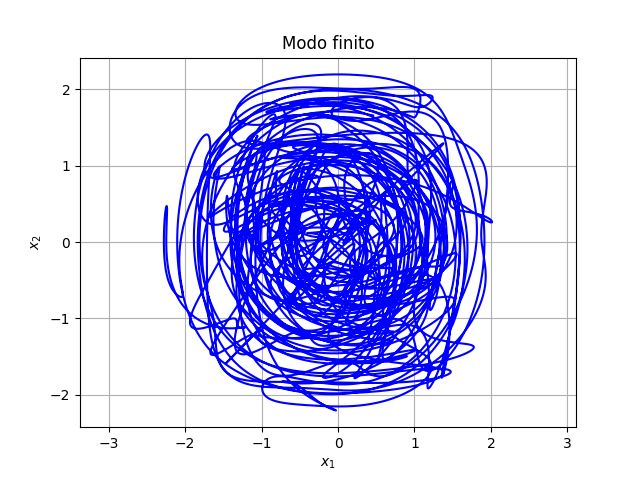
\includegraphics[scale =0.8]{FiniteMode1.png}
\caption{Plot de la trayectoria en el espacio de fase de las coordenadas $x_{1}$ y $x_{2}$ para un tiempo de $0<t<200$ con condiciones iniciales 
$x_{1}(0) = 0540323$, $x_{2}(0) = -1.543569$ ,$x_{3}(0) = -0.680421$ ,$x_{4}(0) = -1.185361$ ,$x_{5}(0) = -0.676307$
estas trayectorias se determinaron numéricamente con un esquema Euler hacia adelante  de primer orden (El desarrollo del esquema numérico se puede encontrar en Github siguiendo este  \href{https://github.com/GoSAUN/Hartmann/tree/master/Codes/FiniteMode}{link})}
\label{FiniteModel}
\end{figure}

\noindent Se puede ver que cada punto en el espacio de fase es inestable, en este caso el sistema es fuertemente mezclado, por tanto preserva la hipótesis de ergodicidad dada por el Teorema de Birkoff, esto significa que cada estado en el espacio de fase dura , en promedio, la misma cantidad de tiempo en todo los lugares del volumen en este espacio. Esto es de gran ayuda dado que el estudio de una sola órbita da una idea general del sistema para cualquier trayectoria.

\subsection{Problemas con las ecuaciones de Navier Stokes}

\noindent Las ecuaciones de Navier Stokes estudiadas en la sección anterior \eqref{NS}  son el punto de partida para el estudio de la turbulencia. Se sabe que en principio no se tiene una ecuación de estado para poder tener completo el sistema de ecuaciones diferenciales, sin embargo el campo de presiones no satisface ninguna ecuación solamente sirve como una condición para preservar la condición de incompresibilidad para cualquier tiempo, Tomando la divergencia de \eqref{NS}, se tiene 

\begin{eqnarray}
\frac{\partial p}{\partial x_{i}\partial x_{i}} = -\frac{\partial}{\partial x_{i}}\left(u_{k}\frac{\partial u_{i}}{\partial x_{k}}\right)
\end{eqnarray}

\noindent entonces la presión es determinada a cada instante de tiempo por el campo global de velocidades, solucionando una ecuación de Poisson, teniendo en cuenta que el efecto instantáneo de las regiones distantes en el flujo local a través de la presión se dan solamente en el límite de la velocidad Mach cero, o de manera equivalente a una velocidad del sonido en el fluido infinita. Se puede ver el siguiente manejo algebraico de las ecuaciones de NAvier Stokes incompresibles para entender mejor la anterior idea

\begin{eqnarray}
\frac{d}{dt}\frac{1}{2}\int_{V}|v|^{2}d\vec{x} = -\nu\int_{V}\frac{\partial u_{\alpha}}{\partial x_{\beta}\partial x_{\beta}}d\vec{x}  
\end{eqnarray}

\noindent donde $V$ es el volumen ocupado para el fluido. Esta relación se relaciona con el balance energético global en el fluido, se puede ver que el término convectivo $u_{k}\frac{\partial u_{i}}{\partial x_{k}}$ y el término de presión $\frac{\partial p}{\partial x_{i}}$  de manera separa conservan la energía total, mientras que el termino viscoso disipa energía en cuanto $\nu > 0$. La anterior ecuación evidencia que todos lo movimientos en una dominio finito debe cesar cuando $t\rightarrow\infty$ siempre y cuando no exista fuerzas externas. 

\noindent Las matemáticas para afrontar las ecuaciones de Navier-Stokes no están desarrolladas completamente, dado que no existe una solución general ni única. Por ahora so se puede trabajar sobre  la extrema simplificación que se hace al trabajar en fluidos ideales. Se plantea el sistema de estudio en un espacio infinito y sujetas a condiciones de decaimiento rápido en las condiciones iniciales 
\begin{eqnarray}
\label{regularidad}
\left|\frac{\partial^{\alpha}u_{o,t}}{\partial x}\right| &\leq& C_{\alpha,K}(1+|x|)^{K}, \qquad \forall \alpha, \ \forall K\\
\left|\frac{\partial^{\alpha}}{\partial x}\frac{\partial^{m}}{\partial t}\vec{F}(\vec{r})\right| &\leq& C_{\alpha,m,K}(1+|x|+t)^{K}, \qquad \forall \alpha, \ ,\forall \beta \forall K
\end{eqnarray}

\noindent y se consideran admisibles las soluciones clásicas de $\vec{u},p,\rho\in C^{\infty}(\rm I\!R\times(0,T))$ que cumplen 

\begin{eqnarray}
\int u^{2}(\vec{r},t)d\vec{r} < \infty\qquad \forall t
\end{eqnarray}

\noindent Esto sugiere que en todo el sistema la energía cinética está acotada. En este punto surge un problema de decisión en cuanto a la manera de resolver el sistema de Navier Stokes

\begin{itemize}
    \item \textbf{Problema de existencia y regularidad:} Se elige $\nu > 0$ y no se consideran fuerzas externas, además se supone que las condiciones iniciales cumplen las condiciones de regularidad \eqref{regularidad} , compresibilidad y decrecimiento rápido en el infinito. Demostrar que existe $\vec{u},\rho\in C^{\infty}(\rm I\!R^{n}\times(0,\infty))$, con energía cinética finita , que resuelve el sistema de ecuaciones de Navier-Stokes en el sentido clásico y $\vec{u}$ y toma el valor de la condición inicial. 
    
    
    
    \item \textbf{Problema colapso de la solución:} Se elige $\nu>0$, encontrando un dato inicial $\vec{u}_{o]}$ y una función que agrupe las fuerzas externas del sistema, tales que no existe una solución clásica de los campos asociados del sistema de ecuaciones de Navier-Stokes 
    
    \item \textbf{Problema de unicidad:} Dada un conjunto de soluciones aceptables físicamente, demostrar que la solución es única durante el tiempo de existencia considerado en el sistema 
    
\end{itemize}

\noindent Se trata entonces principalmente de un problema de decisión tenemos varias opciones. Sí se asume que $T=\infty$ por un tiempo pequeño entonces la solución existe y es regular. Esto fue demostrado por Lery en 1933. Ahora si $\vec{u}_{o}$ es fuertemente oscilante también es regular y existe la solución, sin embargo si el problema del colapso de la solución fuese cierto y una solución no pudiera ser calculada más allá de un tiempo $T>0$, entonces la velocidad se debe hacer infinita cuando $t\rightarrow T$, por tanto es una contrariedad física, dado que la energía sería infinita. Este tópico es un tema de investigación de vanguardia dado que no se tiene unicidad para las soluciones de sistemas físicos que involucren las ecuaciones de Navier-Stokes.

\subsection{Escalas de Turbulencia }

\noindent Se considera un flujo completamente turbulento con un número de Reynolds\footnote{Se recuerda que el número de Reynolds está dado por $R = \frac{\mathcal{U}\mathcal{L}}{\nu}$} alto con una velocidad característica $\mathcal{U}$ y longitud característica $\mathcal{L}$. EL primer concepto que se va a considerar que que la turbulencia puede entenderse como una composición de remolinos con diferentes tamaños.
El tamaño de los remolines está dado por una longitud característica $l_{o}$ la cual es comparable con la escala de fluido $\mathcal{L}$y con una velocidad característica $u(l_{o})$ la cual es comparable con $\mathcal{U}$ ademas con número de Reynolds $Re_{o} = u_{o}l_{o}/\nu$.(que es largo comparado con $Re$).

\medskip

\noindent Richardson fue el primero en proponer la idea de la cascada de energía, esta noción consiste en plantear que los remolinos grandes son inestales y se rompen, transfiriendo energía a remolinos más pequeños. Estos remolinos más pequeños también tienden a romperse y seguir transportando energía a otro mas pequeños aún, esto es el concepto denominado \emph{Cascada de energía}, en la cual la energía se transmite sucesivamente de remolinos grandes a los más pequeños. La tasa de disipación $\varepsilon$ es determinada por el primer proceso en la secuencia de cascada, la cual es del orden $\sim u_{o}^{2}$ y en la escala del tiempo $\sim l_{o}/u_{o}$, entonces la tasa de transferencia de energía se supone como $u_{o}^{2}/\tau = u_{o}^{3}/l_{o}$ independiente de $\nu$ (siempre con la consideración de número de Reynolds alto).

\medskip

\noindent Para empezar a considerar la hipótesis de Kolmogorov empezando por la pregunta ¿Cual es la longitud característica del remolino más pequeño al cual se le tranfiere energía de uno más grande? Como $l_{o}$ decrece, ¿esto hace que $u(l_{o})$ y $\tau(l_{o})$?. Estas preguntas las trató Kolmogorov que respondió a través de tres hipótesis. La primera hipótesis está relacionada con la isotropía de los movimientos de pequeña escala, en general los remolinos grandes son afectados por las condiciones de frontera y son anisotrópicos, Kolmorogov asegura que la anisotropía se pierde en el proceso de reducción de escala entre remolinos grandes a pequeños

\medskip

\hangindent=0.7cm \textbf{Hipótesis de isotropía local: } A un numero de Reynolds Suficientemente alto, las escalas pequeñas en el movimiento turbulento es estadísticamente isotrópico $(l<<l_{o})$

\noindent en este caso se entiende la escala pequeña bajo la definición $l_{p} \approx (1/6)l_{o}$ \cite{pope}\footnote{Justo acá se hace la deducción de este criterio utillizando el tensor del espectro de la velocidad} como el límite entre las escalas grandes donde se tiene anisotropía en los remolinos y las pequeñas donde se tiene isotropía. Kolmogorov argumenta que las esclas grandes pierden energía pasando está a manera de cascada hacia escalas más bajas, la información sobre la geometría de los grandes remolinos se determina por el campo de velocidades y las condiciones de frontera. 

\medskip

\hangindent=0.7cm \textbf{Primera hipótesis de similaridad de Kolmogorov: }En cada flujo turbulento con un número de Reynolds suficientemente alto , la estadística del movimiento de las pequeñas escalas tiene una forma universal única determinada por $\nu$ y $\varepsilon$

\medskip

\noindent El rango de longitud $l<l_{p}$ está relacionado con una categoría de equilibrio universal, en tal rango las escalas de tiempo del fluido, caracterizadas por $l/u(l)$, son pequeñas comparadas con $l/u_{o}$, de tal manera que los pequeños remolinos se adaptan rápidamente para mantener el equilibrio en la transferencia de energía desde las escalas más altas. Dados los dos parámetros $\varepsilon$ y $\nu$  existen unos parámetros únicos de longitud, velocidad y tiempo que pueden ser formados. Estos son

\begin{eqnarray}
\eta &=& \left(\frac{\nu^{3}}{\varepsilon}\right)^{1/4}\\
u_{\eta} &=& (\varepsilon\nu)^{1/4}\\
\tau_{\eta}&=&\left(\frac{\nu}{\varepsilon}\right)^{1/2}
\end{eqnarray}

\noindent dos identidades provenientes de la definiciones anteriores indican que las escalas de Kolmogorov se caracterizan por ser muy pequeñas. El número de Reynolds basado en las escalas de Kolmogorov se define como la unidad, es decir, $\eta u){\eta}\nu=1$, que es consistente con la noción de cascada . Por tanto la la tasa de disipación está dada por 

\begin{eqnarray}
\varepsilon = \nu\left(u_{\eta}\eta\right)^{2}=\frac{\nu}{\tau_{\eta}^{2}}
\end{eqnarray}

\noindent se evidencia que $(u_{\eta}/\eta)=1$. Las relaciones de las escalas pequeñas y grandes están determinadas por las siguientes definiciones , utilizando el hecho $\varepsilon \sim u_{o}^{3}/l_{o}$

\begin{eqnarray}
\frac{\eta}{l_{o}}\sim Re^{-3/4},\qquad \frac{u_{\eta}}{u_{o}}\sim Re^{-1/4},\qquad
\frac{\tau_{\eta}}{\tau_{o}}\sim Re^{-1/2}
\end{eqnarray}

\noindent entonces se ve que para números de Reynolds altos , las velocidades y tiempo de los remolinos pequeños $u_{\eta}$, $\tau_{\eta}$ son chicos en comparación con los grandes, caracterizados por $u_{o}$ y $\tau_{o}$.

\medskip

\hangindent=0.7cm \textbf{Segunda hipótesis de similaridad de Kolmogorov: }En cada flujo turbulento con un número de Reynolds suficientemente alto ,la estadística del movimiento de escala $l$ en el rango  $l_{o}\gg l \gg\eta$ tiene una forma universal que es determinada unicamente por $\varepsilon$ in tependiente de $\nu$

\medskip

\noindent De igual manera que en el anterior análisis de la primera hipótesis de Kolmogorov se define una longitud de escala dada por $l_{d} = 60\eta$, entonces se trabajara bajo la siguiente región $l_{p}>l>l_{d}$. Esta longitu de escala $l_{d}$ ...





\subsection{El espectro de energía}


\noindent Queda por estar determinado como la energía cinética turbulenta está distribuida en los remolinos de diferentes tamaños. Considerando una turbulencia homogénea y considerando un función del espectro de energía $E(k)$, la dinámica del movimiento se caracteriza por el número de onda  $k=2\pi/l$ y el rango de números de onda en el cual el sistema se encuentra 

\begin{eqnarray}
\varepsilon_{(k_{a},k_{b})} = \int_{k_{a}}^{k_{b}}E(k)dk
\end{eqnarray}

\noindent A partir de esta integral se puede encontrar la tasa de disipación \cite{pope} $\varepsilon$ para el movimiento en el rango de numero de onda $(k_{a},k_{b})$, y está dada por 

\begin{eqnarray}
\varepsilon_{(k_{a},k_{b})} = \int_{k_{a}}^{k_{b}}2\nu k^{2}E(k)dk
\end{eqnarray}

\noindent Se considera entonces que la función del espectro de energía  cumple una ley de otencias dada de la siguiente manera

\begin{eqnarray}
E(k) = Ak^{-p}
\end{eqnarray}

\noindent donde $A$ y $p$ son constantes. La energía contenida en los número de onda mayor a $k$ son 

\begin{eqnarray}
k_{k,\infty} = \int_{k}^{\infty}E(k')dk' =\frac{A}{p-1}k^{-(p-1)}
\end{eqnarray}

\noindent para el caso de $p>1$ la integral converge, mientras que para $p<1$ diverge. De manera análoga se tiene para la disipación 

\begin{eqnarray}
\varepsilon_{(0,k)}= \int_{0}^{k}2\nu (k')^{2}E(k')dk'=\frac{2\nu A}{3-p}k^{3-p}
\end{eqnarray}

\noindent para $p<3$, pero la integral diverge para valores $p\geq 3$, entonces , p = 5/3 corresponde al espectro de Kolmogorov para el cual las dos integrales convergen. La cantidad de energía en los altos números de onda decrece como $k\sim k^{-2/3}$ a medida que $k$ aumenta, por otra parte la disipación en los número de onda bajos decrese como $\varepsilon \sim k^{-4/3}$ mientras que k va hacia cero. La primera hipótesis de similaridad de Kolmogorov asegura que $k>k_{p} = 2\pi/l_{p}$. Para la segunda hipótesis se tiene que el espectro de energía es

\begin{eqnarray}
E(k) = C\varepsilon^{2/3}k^{-5/3}
\end{eqnarray}

\noindent donde $C$ es una constante universal



\newpage
\chapter{Teoría de Boltzmann}


El objetivo de la teoría cinética es describir las propiedades macroscópicas de los gases, tales como: presión, temperatura, conductividad térmica, viscosidad, etc; a partir de variables microscópicas que componen los gases como la velocidad, energía cinética e interacción entre otras. Los fundamentos de la teoría moderna fueron establecidos por Maxwell, quien propuso modelos estadísticos y un concepto de ecuación de transporte para poder modelar el comportamiento macroscópico. Esta teoría obtuvo un nuevo impulso a finales del siglo XIX con el trabajo de Boltzmann, quien propuso una ecuación integro-diferencial (ecuación de Boltzmann) la cual representa la evolución de la función de distribución en el espacio de fase. 

\medskip

\noindent Se consideran, en este trabajo, gases compuestos por una gran cantidad de moléculas las cuales se mueven independientemente unas de otras y colisionan entre sí o con las paredes del contenedor. Se asume también que las energías de interacción entre partículas son despreciables en comparación con sus energías cinéticas.

\section{Espacio de fase}

Para definir el espacio de fase se consideran N partículas en tres dimensiones con coordenadas generalizadas $q_{1}, ..., q_{3N}$ y momentos canónicamente conjugados  $p_{1}, ... , p_{3N}$. Llamamos espacio de fase $\Gamma$, al espacio que abarca $6N$ coordenadas. En este espacio, el estado del sistema a un tiempo dado $t$, es representado por un punto a partir de $6N$ valores, $3N$ debido a las componentes del vector de posición y $3N$ de las velocidades de las $N$ partículas.

\medskip

\noindent Generalmente los sistemas físicos que se estudian en la naturaleza se componen de una gran cantidad de partículas, de esta manera el espacio de fase tiene muchas dimensiones y es muy difícil determinar un punto en $\Gamma$. Para simplificar el estudio de la física a nivel macroscópico es necesario calcular cantidades como la energía, el volumen, etc. Estas se calculan conociendo un gran numero de micro estados, es decir, una colección de muchos puntos en el espacio de fase, sin embargo no será posible encontrar todos los micro estados y se hace necesario caracterizarlos mediante una función de distribución, adoptando una visión probabilística en $\Gamma$. 

\medskip

\noindent Un punto en el espacio de fase se escribe como $(q,p) = (q_{1}, ... ,q_{3N}, p_{1}, ... ,p_{3N})$ y se considera una densidad de probabilidad de ocurrencia en el tiempo t como $f(q,p,t)$. Esta distribución de probabilidad describe propiedades estadísticas de los estados en $\Gamma$ y permite analizar casos microscópicos dentro de resultados macroscópicos. En adelante el desafío será encontrar la función de distribución correspondiente a la situación física  particular. (\textbf{label seccion)}.

\medskip

\noindent Para un gran número de partículas N tenemos \cite{Schwabl}

\begin{eqnarray}
f(q,p,t)dqdp = f(q_{1}, ... , q_{3N},p_{1},..,p_{3N},t)\prod_{i=1}^{3N}dq_{i}dp_{i},
\end{eqnarray}

\noindent que representa la probabilidad de encontrar un sistema en un tiempo $t$, con un volumen en el espacio de fase $dqdp$, en la vecindad del punto $(q,p)$ en el espacio $\Gamma$. $f(q,p,t)$ es llamada la \textbf{función de distribución}, la cual debe ser positiva $f(q,p,t) \geq 0$ y normalizable. 

\begin{eqnarray}
f = f(\vec{r},\vec{v},t) \qquad f:{\rm I\!R}^{3}\times{\rm I\!R}^{3}\times{\rm I\!R}^{+}\longrightarrow{\rm I\!R}^{+}
\end{eqnarray}

%\section{Teorema de Louville}
%Se quiere determinar la dependencia temporal de la función de distribución 
%f(q,p,t), supongamos una distribución inicial $f(q_{o},p_{o})$ en $t = 0$


\section{Función de distribución de Maxwell}

La principal pregunta es, ¿cómo conocer la probabilidad de encontrar una molécula que se mueve en un rango de velocidades $\vec{v}+d\vec{v}$? Para poder responder tal pregunta se consideran tres suposiciones físicas \cite{lecture2}

\begin{itemize}
    \item[$\mathbf{\bullet}$] El número de partículas con velocidad $\vec{v}$ es proporcional a $d\vec{v}$. Entonces se considera que $\phi(\vec{v})d\vec{v}$ representa la probabilidad de encontrar una molécula con velocidad $\vec{v}$ en un rango $\vec{v} + d\vec{v}$
    
    \item[$\mathbf{\bullet}$] La probabilidad de encontrar partículas con velocidad $\vec{v}$ es independiente de los grados de libertad (en cada coordenada)

    \begin{eqnarray}
    \phi(u)du\ \phi(v)dv\ \phi(w)dw,
    \end{eqnarray}
    
    entonces se define una función de distribución que depende de las probabilidades de la siguiente manera
    
    \begin{eqnarray}
    f(u,v,w)dudvdw = n\phi(u)du\phi(v)dv\phi(w)dw,
    \end{eqnarray}
    
    donde $n$ denota la densidad de partículas dentro del diferencial del espacio de fase.
    
    \item[$\mathbf{\bullet}$] \textbf{Hipótesis de isotropía:} En el proceso de equilibrio, en ausencia de fuerzas externas, no se distingue entre las tres direcciones, es decir, se asume que las funciones de distribución tridimensionales se componen del producto de tres funciones unidimensionales
    
    \begin{eqnarray*}
    f(u,v,w) = n\phi(u)\phi(v)\phi(w) =\Phi(|\vec{v}|),
    \end{eqnarray*}
    
    entonces se toma el logaritmo para obtener
    
    \begin{eqnarray*}
    \ln \Phi(|\vec{v}|) = \ln n + \ln\phi(u)+\ln\phi(v)+\ln\phi(w),
    \end{eqnarray*}
    
    derivando para cada componente se obtiene un resultado interesante, que impone una condición de vital importancia
    
    
    \begin{eqnarray}
    \frac{1}{|\vec{v}|}\frac{d\ln\Phi(|\vec{v}|)}{d|\vec{v}|} = \frac{1}{u}\frac{d(\ln\phi(u))}{du}=\frac{1}{v}\frac{d\ln\phi(v)}{dv}=\frac{1}{w}\frac{d\ln\phi(w)}{dw},
    \end{eqnarray}
    
    la única posibilidad para que se cumplan las anteriores relaciones es que cada una sea igual a una constante. Integrando se llega a la siguiente expresión 
    
    \begin{eqnarray}
    \label{Fdistribucion}
    \phi(|\vec{v}|) = \alpha^{3} e^{-\beta v^{2}} \qquad\qquad  f(u,v,w) = n\alpha^{3}e^{-\beta v^{2}}
    \end{eqnarray}
    
    donde $\alpha$ y $\beta$ son constantes de integración postivas. Se elige negativo el exponente para que la función sea normalizable, es decir, sea una función de decreciemiento rápido, ideal para la descripción de cantidades físicas \cite{strichartz}.
    
    Ahora se determinan las constantes de integración en el equilibrio termodinámico, y así las variables de estado que se  utilizan son la densidad $\rho$ y la densidad de energía interna $\rho\epsilon$. 
    
    \begin{eqnarray}
    \label{rho}
    \rho(\vec{r},t) &=& mn = \int_{{\rm I\!R^{3}}}mf(\vec{r},\vec{v},t)d\vec{v}\\
    \label{denener}
    \rho(\vec{r},t)\epsilon &=& \frac{3}{2}nKT=\int_{{\rm I\!R^{3}}}\frac{1}{2}mv^{2}f(\vec{r},\vec{v},t)d\vec{v}
    \end{eqnarray}
    
    la ecuación \eqref{denener} expresa que la energía cinética de traslación promedio  por partícula está dada por el teorema de la equipartición de la energía. Integrando las anteriores expresiones y utilizando \eqref{Fdistribucion} se llega a las siguientes relaciones \footnote{Para calcular las integrales de la teoría cinética se puede utilizar la función Gamma 
    \begin{eqnarray}
    \int_{0}^{\infty}x^{n}e^{-\alpha x^{2}}dx = \frac{1}{2}\Gamma\left(\frac{n+1}{2}\right)\left(\frac{1}{\alpha}\right)^{\frac{n+1}{2}}
    \end{eqnarray}
     }
     
     \begin{eqnarray}
     \label{calculoint}
     \rho = \rho\alpha^{3}\left(\frac{\pi}{\beta}\right)^{3/2} , \qquad \frac{3}{2}nkT =\frac{3}{4}mn\alpha^{3}\left(\frac{\pi}{\beta}\right)^{3/2} \frac{1}{\beta}
     \end{eqnarray}
     
     encontrando,  a partir de las relaciones \eqref{calculoint},
     
     \begin{eqnarray}
     \boxed{
     \alpha = \left(\frac{m}{2\pi kT}\right)^{1/2}, \qquad \beta=\frac{m}{2kT}
     }
     \end{eqnarray}
    
    
    por lo tanto la función de distribución está dado por la siguiente expresión 
    
    \begin{eqnarray}
    f(\vec{r},\vec{v},t) = \rho(\vec{r},t)\left(\frac{m}{2\pi kT}\right)^{3/2}e^{-mv^{2}/2kT}.
    \end{eqnarray}

\end{itemize}

\noindent Esta es la distribución de Maxwell-Boltzmann , que modela la evolución en el tiempo de cada partícula en una posición y velocidad en particular. Sí se conoce $f$, las cantidades macroscópicas observables pueden calcularse a partir de funciones microscópicas. En particular se tienen los momentos macroscópicos  \cite{lecture1}

\begin{eqnarray}
\rho(\vec{r},t)&=&mn(\vec{r},t)=m\int_{{\rm I\!R}^{3}}f(\vec{r},\vec{v},t)d\vec{v}\\
\vec{u}(\vec{r},t) &=& \frac{1}{n(\vec{v},t)}\int_{{\rm I\!R}^{3}}\vec{v} f(\vec{r},\vec{v},t)d\vec{v}
\end{eqnarray}

\noindent que son respectivamente la densidad de masa y la densidad de velocidad. Ahora definimos la energía traslacional de la forma

\begin{eqnarray}
\epsilon(\vec{r},t)=\frac{1}{n(\vec{r},t)}\int_{{\rm I\!R}^{3}}(\vec{v}-\vec{u})^{2}f(\vec{r},\vec{v},t)d\vec{v}
\end{eqnarray}




\section{Ecuación de Boltzmann}



\noindent La función de distribución $f$ depende  de $\vec{x}$, $\vec{\xi}$ y $t$. Veamos su variación temporal

\begin{eqnarray}
\frac{df}{dt} = \left(\frac{\partial f}{\partial x_{\alpha}}\right)\frac{dx_{\alpha}}{dt}+\left(\frac{\partial f}{\partial \xi_{\alpha}}\right)\frac{d\xi_{\alpha}}{dt}+\left(\frac{\partial f}{\partial t}\right)
\end{eqnarray}

\noindent En donde $dx_{\alpha}/dt$ es la velocidad de las partículas a nivel mesoscópico $\xi_{\alpha}$. Por otro lado, el segundo término está relacionado con la aceleración y así, teniendo en cuenta la segunda ley de Newton, podemos escribir la densidad de fuerza como $d\xi_{\alpha}/dt = F_{\alpha}/\rho$. Por lo tanto la ecuación de evolución que tenemos está dada por 

\begin{eqnarray}
\frac{df}{dt} = \xi_{\alpha}\left(\frac{\partial f}{\partial x_{\alpha}}\right)+\frac{F_{\alpha}}{\rho}\left(\frac{\partial f}{\partial \xi_{\alpha}}\right)+\frac{\partial f}{\partial t}
\end{eqnarray}

\noindent en general, el lado izquierdo de la ecuación es un término fuente que indica la tasa de cambio de la función de distribución dada por las colisiones entre partículas.  La siguiente ecuación es llamada \emph{Ecuación de Boltzmann}

\begin{eqnarray}
\label{Boltzmann}
\frac{\partial f}{\partial t} + \xi_{\alpha}\left(\frac{\partial f}{\partial x_{\alpha}}\right)+\frac{F_{\alpha}}{\rho}\left(\frac{\partial f}{\partial \xi_{\alpha}}\right)=\Omega(f)
\end{eqnarray}

\noindent donde se ha definido el operador de colisión al termino $\Omega(f)$ el cual puede tener diversas formas, existe un amplio campo de investigación al respecto \cite{lecture3}\cite{lecture4}\cite{lecture5}. Sin embargo debemos exigir a tal operador que conserve tres cantidades físicas importantes, la masa, el momento y la energía. Matemáticamente se expresan como sigue 

\begin{eqnarray}
\int\Omega(f)d\vec{\xi} = 0 \qquad \int\vec{\xi}\Omega(f)d\vec{\xi} = 0 \qquad \int\xi^{2}\Omega(f)d\vec{\xi} = 0.
\end{eqnarray}

\noindent para deducir el operador de colisión se necesita resolver dos  integrales complicadas sobre todo el espacio \cite{lecture5}, que en esencia es considerar todas las posibles formas de colisión que puedan tener las partículas en estudio para una fuerza en particular. Un operador que cumple con tales condiciones fue el propuesto por Bhatnagar, Gross y Krook en 1954 \cite{BGK}, entonces se asume que 

\begin{eqnarray}
\Omega(f) = -\frac{1}{\tau}(f-f^{(0)})
\end{eqnarray}

\noindent en la anterior ecuación $\tau$ es el tiempo de relajación, el cual cuantifica que tan rápido chocan las partículas 

\section{Ecuaciones de conservación macroscópicas}

\noindent Tomando los momentos de la ecuación de Boltzmann \eqref{Boltzmann} se pueden encontrar las ecuaciones de conservación del sistema tales como la masa, el momento y la energía. Se define entonces

\begin{eqnarray}
\label{momentos}
\Pi_{o} = \int f d\vec{\xi} = \rho &\qquad& \Pi_{\alpha} = \int \xi_{\alpha}f d\vec{\xi} = \rho u_{\alpha}\\
\Pi_{\alpha\beta} = \int \xi_{\alpha\beta}f d\vec{\xi}  &\qquad& \Pi_{\alpha\beta\gamma} = \int \xi_{\alpha}\xi_{\beta}\xi_{\gamma}f d\vec{\xi} \nonumber
\end{eqnarray}

\noindent Para la conservación de la masa se integra \eqref{Boltzmann} obteniendo. 

\begin{eqnarray}
\frac{\partial}{\partial t}\int f d\vec{\xi}+\frac{\partial}{\partial x_{\alpha}}\int \xi_{\alpha}fd\vec{\xi}+\frac{F_{\alpha}}{\rho}\int \frac{\partial f}{\partial \xi_{\alpha}}d\vec{\xi} = \int \Omega(f)d\vec{\xi}
\end{eqnarray}

\noindent Notando que $t$ y $x$ no son funciones de $\xi$, podemos permutar la integral con la divergencia y reorganizar términos. Falta hacer el calculo del término de fuerza utilizando la integración por partes multidimensional\footnote{Ecuacion de integración por partes multidimensional \begin{eqnarray}
\label{partes}
\int_{V} \frac{\partial u}{\partial x_{\alpha}} = \int_{S}uv dS_{\alpha} - \int_{V}u\frac{\partial v}{\partial x_{\alpha}}\nonumber
\end{eqnarray}
} y asumiendo que las integrales de superficie se desvanecen cuando $\vec{\xi}\rightarrow  0$. Se impone esta última condición para asegurar que las ecuaciones de conservación sean finitas. Entonces se llega a la siguiente ecuación utilizando \eqref{momentos}


\begin{eqnarray}
\boxed{\frac{\partial \rho}{\partial t} +\frac{\partial \rho u_{\alpha}}{\partial x_{\alpha}}= 0 }
\end{eqnarray}

\noindent que es la ecuación de continuidad \cite{Landau}. La importancia de este resultado radica en que la forma de la ecuación de continuidad se mantendrá sin importar la forma funcional especifica de la función distribución, de tal manera que la definición de los momentos en la ecuación tienen mayor relevancia debido a que conectan el mundo mesoscópico con las ecuaciones macroscópicas.

\medskip

\noindent Para el caso de la siguiente ecuación de conservación se toma el primer momento de \eqref{Boltzmann} y se hace la integral en todo el espacio de velocidades, obteniendo la siguiente relación 



\begin{eqnarray}
\frac{\partial}{\partial t}\int \xi_{\alpha}f d\vec{\xi}+\frac{\partial}{\partial x_{\beta}}\int \xi_{\alpha}\xi_{\beta}fd\vec{\xi}+\frac{F_{\beta}}{\rho}\int \xi_{\alpha}\frac{\partial f}{\partial \xi_{\beta}}d\vec{\xi} = \int \xi_{\alpha}\Omega(f)d\vec{\xi}
\end{eqnarray}

\noindent Se utiliza la integración por partes para encontrar el momento relacionado con el término de la fuerza, encontrando que se puede hacer 

\begin{eqnarray}
\int \xi_{\alpha}\frac{\partial f}{\partial \xi_{\beta}}d\vec{\xi} = -\int \frac{\partial \xi_{\alpha}}{\partial \xi_{\beta}}fd\vec{\xi}= -\rho\delta_{\alpha\beta}
\end{eqnarray}

\noindent como resultado podemos ver la ecuación de conservación del momento dada por la siguiente expresión 

\begin{eqnarray}
\frac{\partial (\rho u_{\alpha})}{\partial t}+\frac{\partial \Pi_{\alpha\beta}}{\partial x_{\beta}} = F_{\alpha}
\end{eqnarray}

\noindent dada la definición de $\Pi_{\alpha\beta}$ dada en \eqref{momentos} podemos entender físicamente como el flujo de cantidad de movimiento dirección $\alpha$ de la dirección $\beta$ de momento, en donde se evidencia que es simétrica respecto de índices. Veamos con más detalle $\Pi_{\alpha\beta}$ , definamos $\xi_{\alpha}\xi_{\beta}=(u_{\alpha}+v_{\alpha})(u_{\beta}+v_{\beta})$, entonces obtenemos lo siguiente 

\begin{eqnarray}
\Pi_{\alpha\beta} = \int (u_{\alpha}u_{\beta}+u_{\alpha}v_{\beta}+v_{\alpha}u_{\beta}+v_{\alpha}v_{\beta})fd\vec{\xi} = \rho u_{\alpha}u_{\beta} -\sigma_{\alpha}
\end{eqnarray}

\noindent tomando la condición de simetría de el primer momento $\Pi_{\alpha\beta}=\Pi_{\beta\alpha}$ se encuentra  que $u_{\alpha}v_{\beta} + v_{\alpha}u_{\beta}=0$, esto hace que los términos intermedios de la anterior integral se cancelen, obteniendo los dos términos de la do derecho bajo esta definición de $\sigma$

\begin{eqnarray}
\sigma_{\alpha\beta} = - \int v_{\alpha}v_{\beta}fd\vec{\xi}
\end{eqnarray}

\noindent el cual representa la difusión del momento y está determinado por la forma que se eliga de f, finalmente se tiene

\begin{eqnarray}
\boxed{\frac{\partial (\rho u_{\alpha})}{\partial t}+\frac{\partial(\rho u_{\alpha}u_{\beta})}{\partial x_{\beta}}=\frac{\partial \sigma_{\alpha\beta}}{\partial x_{\beta}}+F_{\alpha}}
\end{eqnarray}

\noindent como última consideración encontramos la ecuación de conservación de energía , tomando el segundo momento de la función de distribución de la ecuación de Boltzmann \eqref{Boltzmann}

\begin{eqnarray}
\frac{\partial}{\partial t}\int \xi_{\alpha}\xi_{\beta}f d\vec{\xi}+\frac{\partial}{\partial x_{\alpha}}\int \xi_{\alpha}\xi_{\beta}\xi_{\gamma}fd\vec{\xi}+\frac{F_{\alpha}}{\rho}\int \xi_{\alpha}\xi_{\beta}\frac{\partial f}{\partial \xi_{\alpha}}d\vec{\xi} = \int \xi_{\alpha}\xi_{\beta}\Omega(f)d\vec{\xi}
\end{eqnarray}

\noindent que por las definiciones de momentos \eqref{momentos} encontramos una ecuación de conservación del siguiente estilo 


\begin{eqnarray}
\frac{\partial (\rho E)}{\partial t} + \frac{1}{2}\frac{\partial \Pi_{\alpha\beta\gamma}}{\partial x_{\alpha}}=F_{\alpha}u_{\alpha}
\end{eqnarray}

En donde $\Pi_{\alpha\beta\gamma}$ representa el flujo de energía en la dirección $\alpha$. Tomando en cuenta el desarrollo en la deducción de el primer momento, calculamos 

\begin{eqnarray}
\frac{1}{2}\Pi_{\alpha\beta\gamma}&=&\frac{1}{2}\int (u_{\alpha}u_{\beta}u_{\gamma}+u_{\alpha}u_{\beta}u_{\gamma}+u_{\alpha}u_{\beta}u_{\gamma}+u_{\alpha}u_{\beta}u_{\gamma})fd\vec{\xi}\nonumber\\
&=&\frac{1}{2}\rho u_{\alpha} u^{2}+\rho u_{\alpha}e- u_{\beta}\sigma_{\alpha\beta}+q_{\alpha}\nonumber\\
&=&\rho u_{\alpha}E - u_{\beta}\sigma_{\alpha\beta} +q_{\alpha}
\end{eqnarray}

\noindent se tiene ahora que el primer término representa la advección macroscópica de la energía, el segundo término como el trabajo hecho por el tensor de "Strain" y se define el último termino como la difusión de la energía de la siguiente manera

\begin{eqnarray}
q_{\alpha} = \frac{1}{2}\int v_{\alpha} v^{2}f d\vec{\xi}
\end{eqnarray}

Finalmente se llega a la ecuación de conservación relacionada con la energía

\begin{eqnarray}
\boxed{
\frac{\partial (\rho e)}{\partial t} + \frac{\partial (\rho u_{\alpha}e)}{\partial x_{\alpha}}= \sigma_{\alpha\beta}\frac{\partial (\sigma_{\alpha\beta}u_{\beta})}{\partial x_{\alpha}}+ F_{\alpha}u_{\alpha}-\frac{\partial q_{\alpha}}{\partial x_{\alpha}}
}
\end{eqnarray}

\newpage










\newpage
\chapter{Magnetohidrodinámica (MHD)}


\noindent El objetivo concreto de este capítulo es dar un entendimiento físico del modelo ideal magnetohidrodinámico (MHD), esto incluye una descripción básica del modelo.
\begin{comment}

\noindent El modelo ideal MHD se sitúa bajo la consideración de longitud de onda larga y bajas frecuencias. En este orden de ideas y pretendiendo abarcar la física desde una perspectiva más formal, en la deducción del caso ideal se consideran principios básicos. Utilizando las ecuaciones de Maxwell\eqref{Leygauss},\eqref{divceroB},\eqref{Ampere},\eqref{FM} y la ecuación de Boltzmann\eqref{Boltzmann},



\begin{eqnarray}
\nabla \cdot \vec{E} &=& \frac{\rho}{\epsilon_{0}}\nonumber\\
\nabla \cdot \vec{B} &=& 0\nonumber\\
\nabla\times\vec{B} &=& \mu_{o}\vec{J}+\frac{1}{c^{2}}\frac{\partial \vec{E}}{\partial t}\nonumber\\
\nabla\times\vec{E} &=& \frac{\partial \vec{B}}{\partial t}\nonumber\\
\label{BMHD}
  \left(\frac{\partial f}{\partial t}\right)_{c} &=&\frac{\partial f}{\partial t} + v_{i}\frac{\partial f}{\partial x_{i}} + \frac{q(E_{i}+\varepsilon_{ijk}v_{j}B_{k})}{m}\frac{\partial f}{\partial v_{i}}
\end{eqnarray}

\noindent en particular para describir los fenomenos MHD se incluye el termino de fuerza de Lorentz, además las definiciones de densidad de corriente y densidad de carga 

\begin{eqnarray}
\vec{J} &=& q\int \vec{\xi}f(\vec{x},\vec{\xi},t)d\vec{\xi}\\
\sigma &=& q\int f(\vec{x},\vec{\xi},t)d\vec{\xi} d\vec{\xi}
\end{eqnarray}

\noindent donde $f$ es la función de distribución definida en la sección anterior. En la descripción de Boltzmann se consideran dos tipos de fuerzas que actúan sobre las partículas. La primera de ellas es de largo alcanze y está dada por las fuerzas de Lorentz $q(\vec{E}+\vec{v}\times\vec{B})$ en la cual $\vec{E}$ y $\vec{B}$ son de buen comportamiento en el sentido del calculo diferencial y obtenidos a partir de el vector densidad de corriente y la densidad de carga. La segunda fuerza está asociadada con el operador de colisión\cite{BGK} impuesto en la ecuación de Boltzmann, el cual es una interacción de corto alcance. Es bueno recordar que nuestro parámetro de comparación será el camino libre medio\cite{lecture5}. 

\medskip

\end{comment}
Asumimos que el fluido no es relativista y el interés se centra en variaciones de tiempo muy lentas, ado esto podemos considerar ignorar la corriente de desplazamiento al tener en cuenta estas consideraciones. Por lo ranto la ley de Ohm\cite{Jackson}:

\begin{eqnarray}
\label{OHMr}
\vec{E}' = \eta\vec{J}
\end{eqnarray}

\noindent donde $\vec{E}'$ es un campo eléctrico visto desde un sistema de referencia con velocidad relativa $\vec{v}$, por lo tanto el campo eléctrico en tal sistema está dado por 

\begin{eqnarray}
\vec{E}' = \frac{\vec{E}+\vec{v}\times\vec{B}}{\sqrt{1-v^{2}/c^{2}}}
\end{eqnarray}

\noindent como el problema no tiene en cuenta efectos de la relatividad especial se considera una expansión de Taylor y se restringe a primer orden la serie

\begin{eqnarray}
\vec{E}' = \vec{E}+\vec{v}\times\vec{B} + \mathcal{O}\left(\frac{v^{2}}{c^{2}}\right)
\end{eqnarray}

\noindent entonces teniendo en cuenta \eqref{OHMr} y \eqref{Ampère} se llega :

\begin{eqnarray}
\vec{E} = -\vec{v}\times\vec{B}+\eta\vec{J} \qquad \qquad \vec{J} = \frac{1}{\mu_{o}}(\nabla \times \vec{B})
\end{eqnarray}

\noindent se puede utilizar la ecuación de Faraday-Maxwell \eqref{FM}, obteniendo:

\begin{eqnarray}
\label{Btemp}
\frac{\partial \vec{B}}{\partial t} &=& -\nabla \times \vec{E} = \nabla \times(-\vec{v}\times\vec{B}+\eta\vec{J)}\\
&=& -\nabla \times (\eta\vec{J})+\nabla\times(\vec{v}\times\vec{B})\\
&=&-\nabla\times\left(\frac{\eta}{\mu_{o}}(\nabla\times\vec{B})\right) + \nabla\times(\vec{v}\times\vec{B})\\
&=&\frac{\eta}{\mu_{o}}\nabla^{2}\vec{B} + \nabla\times(\vec{v}\times\vec{B})
\end{eqnarray}

\noindent con este procedimiento se elimina la dependencia explícita en las ecuaciones del campo eléctrico, la evolución temporal del campo magnético depende de variaciones espaciales de de $\vec{B}$ y del campo de velocidades del sistema. Para hacer un análisis físico más simple se escribe \eqref{Btemp} en forma conservativa, para tal fin se considera el segundo termino de la anterior ecuación

\begin{eqnarray}
\nabla\times(\vec{v}\times\vec{B}) &=& \varepsilon_{ijk}\frac{\partial}{\partial x_{j}}(\varepsilon_{kml}v_{m}B_{l})\\
&=&\varepsilon_{ijk}\varepsilon_{kml}\frac{\partial}{\partial x_{j}}(v_{m}B_{l})\\
&=&-\varepsilon_{ijk}\varepsilon_{lmk}\frac{\partial}{\partial x_{j}}(v_{m}B_{l})\\
&=&(\delta_{il}\delta_{jm}-\delta_{im}\delta_{jl})\frac{\partial}{\partial x_{j}}(v_{m}B_{l})\\
&=&\frac{\partial}{\partial x_{j}}(v_{i}B_{j})-\frac{\partial}{\partial x_{j}}(v_{j}B_{i})\\
&=&\frac{\partial}{\partial x_{j}}(v_{i}B_{j}-v_{j}B_{i})
\end{eqnarray}

\noindent por tanto para el campo magnético  la ecuación de conservación es la siguiente 

\begin{eqnarray}
\boxed{
\frac{\partial B_{i}}{\partial t} + \frac{\partial}{\partial x_{j}}(v_{i}B_{j}-v_{j}B_{i}) = \frac{\eta}{\mu_{o}}\frac{\partial^{2}B_{i}}{\partial x_{j}^{2}}
}.
\end{eqnarray}

%\noindent esta ecuación está acoplada con la ecuación de Euler para dar la evolución de $v$ además actuando como la fuerza externa que da el comportamiento particular de los plasmas


\noindent Ahora se encuentra la ecuación de momento del fluido magnetizado, para esto se estudia el cambio del momento en el tiempo para tal fin se considera la ecuación de continuidad \eqref{continuidad} y la ecuación de Navier Stokes \eqref{NS}. Se escriben de manera conveniente tal y como sigue 

\begin{eqnarray}
\label{contindicial}
\frac{\partial \rho}{\partial t}&=&-\frac{\partial}{\partial x_{k}}(\rho u_{k})\\
\label{NSindicial}
\frac{\partial u_{i}}{\partial t} &=& -u_{k}\frac{\partial u_{i}}{\partial x_{k}} - \frac{1}{\rho}\frac{\partial p}{\partial x_{i}} + \frac{1}{\rho}\frac{\partial \sigma_{ik}}{\partial x_{k}}
\end{eqnarray}



\noindent se adiciona al problema la fuerza de lorentz, de esta manera se incluye la interacción electromagnética. En primer lugar vemos que la variación de momento del fluido está dada por la siguiente expresión 

\begin{eqnarray}
\frac{\partial}{\partial t}(\rho u_{i}) = u_{i}\frac{\partial 
\rho}{\partial t} + \rho \frac{\partial u_{i}}{\partial t} + (\vec{F}_{EM})_{i} 
\end{eqnarray}

\noindent teniendo en cuenta \eqref{contindicial} y \eqref{NSindicial}

\begin{eqnarray}
\frac{\partial}{\partial t}(\rho u_{i}) = u_{i}\left[-\frac{\partial}{\partial x_{k}}(\rho u_{k})\right] + \rho\left[-u_{k}\frac{\partial u_{i}}{\partial x_{k}} - \frac{1}{\rho}\frac{\partial p}{\partial x_{i}} + \frac{1}{\rho}\frac{\partial \sigma_{ik}}{\partial x_{k}}\right] + (\vec{j}\times\vec{B})_{i}\nonumber
\end{eqnarray}

\noindent ahora podemos reescribir un poco la ecuación ayudándonos de una regla de la cadena

\begin{eqnarray}
\frac{\partial}{\partial x_{k}}(\rho u_{i}u_{k}) = u_{k}\frac{\partial(\rho u_{i})}{\partial x_{k}}+u_{i}\frac{\partial(\rho u_{k})}{\partial x_{k}}\nonumber
\end{eqnarray}

\noindent obteniendo

\begin{eqnarray}
\frac{\partial}{\partial t}(\rho u_{i}) = -\frac{\partial}{\partial x_{k}}(\rho u_{i}u_{k})-\frac{\partial p}{\partial x_{k}}\delta_{ik} + \frac{\partial \sigma_{ik}}{\partial x_{k}}+ \left(\frac{1}{\mu_{o}}(\nabla\times\vec{B})\times\vec{B}\right)_{i}\nonumber\\
\label{momentos1}
\frac{\partial}{\partial t}(\rho u_{i})+\frac{\partial}{\partial x_{k}}\left[\rho u_{i}u_{k}+p\delta_{ik}\right] = \frac{\partial \sigma_{ik}}{\partial x_{k}}+\left(\frac{1}{\mu_{o}}(\nabla\times\vec{B})\times\vec{B}\right)_{i}
\end{eqnarray}

\noindent Considerando el segundo termino del lado derecho

\begin{eqnarray}
\left((\nabla\times\vec{B})\times\vec{B}\right)_{i}&=&\varepsilon_{ijk}\left(\varepsilon_{jmn}\frac{\partial B_{n}}{\partial x_{m}}\right)B_{k}\nonumber\\
&=&-\varepsilon_{ikj}\varepsilon_{jmn}\frac{\partial B_{n}}{\partial x_{m}}B_{k}\nonumber\\
&=&(\delta_{im}\delta_{kn}-\delta_{in}\delta_{km})\frac{\partial B_{n}}{\partial x_{m}}B_{k}\nonumber\\
&=&\delta_{im}\delta_{kn}\frac{\partial B_{n}}{\partial x_{m}}B_{k}-\delta_{in}\delta_{km}\frac{\partial B_{n}}{\partial x_{m}}B_{k}\nonumber\\
&=&B_{k}\frac{\partial B_{k}}{\partial x_{i}}-B_{k}\frac{\partial B_{i}}{\partial x_{k}}
\end{eqnarray}

\noindent se toman dos expresiones auxiliares para reescribir en forma de divergencia


    \begin{eqnarray}
    \frac{\partial}{\partial x_{i}}(B_{k}B_{k}) = 2B_{k}\frac{\partial B_{k}}{\partial x_{i}}\quad\longrightarrow\quad \boxed{B_{k}\frac{\partial B_{k}}{\partial x_{i}} = \frac{1}{2}\frac{\partial}{\partial x_{i}}(B_{k}B_{k})}
    \end{eqnarray}
    \begin{eqnarray}
    \frac{\partial}{\partial x_{k}}(B_{i}B_{k}) = B_{k}\frac{\partial B_{i}}{\partial x_{k}} + B_{i}\frac{\partial B_{k}}{\partial x_{k}} \quad\longrightarrow\quad \boxed{B_{k}\frac{\partial B_{i}}{\partial x_{k}}=\frac{\partial}{\partial x_{k}}(B_{i}B_{k})-B_{i}\frac{\partial B_{k}}{\partial x_{k}}}
    \end{eqnarray}

\noindent la fuerza de Lorentz se reescribe de la siguiente manera

\begin{eqnarray}
\left((\nabla\times\vec{B})\times\vec{B}\right)_{i} &=& \frac{\partial}{\partial x_{k}}(B_{i}B_{k})-B_{i}\frac{\partial B_{k}}{\partial x_{k}}-\frac{1}{2}\frac{\partial}{\partial x_{i}}(B_{k}B_{k})\nonumber 
\end{eqnarray}

\noindent como $\nabla\cdot\vec{B} = 0$ la ecuación se reduce a:

\begin{eqnarray}
\label{LorentzIndicial}
\left((\nabla\times\vec{B})\times\vec{B}\right)_{i} &=& \frac{\partial}{\partial x_{k}}(B_{i}B_{k})-\frac{1}{2}\frac{\partial}{\partial x_{i}}(B_{k}B_{k}) 
\end{eqnarray}

Se reemplaza \eqref{LorentzIndicial} en \eqref{momentos1} para obtener

\begin{eqnarray}
\boxed{\frac{\partial(\rho u_{i})}{\partial t}+\frac{\partial}{\partial x_{k}}\left[\rho u_{i}u_{k}+\left(p+\frac{1}{2\mu_{o}}B^{2}\right)\delta_{ik}-\frac{1}{\mu_{o}}B_{i}B_{k}\right] = \frac{\partial \sigma_{ik}}{\partial x_{k}}}
\end{eqnarray}

Donde $B^{2}$ hace referencia al término de presión magnética y el tensor $\vec{B}\vec{B}$ es la tensión magnética. 

\section{Ecuaciones del sistema}

Las ecuaciones fundamentales en MHD empleadas se resumen de la siguiente manera

\begin{eqnarray}
\frac{\partial \rho}{\partial t} + \nabla\cdot(\rho\vec{v}) &=& 0\nonumber\\
\frac{\partial B_{i}}{\partial t} + \frac{\partial}{\partial x_{j}}(v_{i}B_{j}-v_{j}B_{i}) &=& \frac{\eta}{\mu_{o}}\frac{\partial^{2}B_{i}}{\partial x_{j}^{2}}\\
\frac{\partial(\rho u_{i})}{\partial t}+\frac{\partial}{\partial x_{k}}\left[\rho u_{i}u_{k}+\left(p+\frac{1}{2\mu_{o}}B^{2}\right)\delta_{ik}-\frac{1}{\mu_{o}}B_{i}B_{k}\right] &=& \frac{\partial \sigma_{ik}}{\partial x_{k}}\nonumber
\end{eqnarray}




\section{Parámetros adimensionales}
En términos de una velocidad típica del plasma $v_{o}$ y una longitud de escala $l_{o}$, la magnitud del término de convección se define el \emph{Número magnético de Reynolds}
\section{Física Solar }

\newpage
\chapter{Observaciones}

\section{Fotosfera}
\section{Medición}
\section{Resultados}

\newpage
\chapter{Resultados}


\newpage

\newpage\null\thispagestyle{empty}\newpage
%\include{1Definiciones}
%\newpage\null\thispagestyle{empty}\newpage
\newpage


%\include{CAP3}
%\newpage
%\include{CAPFA}










\bibliographystyle{plain}
\bibliography{references}


\end{document}